\documentclass[3p,review,12pt]{elsarticle}
\usepackage{lineno,hyperref,notoccite,etoolbox}
\modulolinenumbers[5]
\makeatletter
\def\ps@pprintTitle{%
	\let\@oddhead\@empty
	\let\@evenhead\@empty
	\def\@oddfoot{\centerline{\thepage}}%
	\let\@evenfoot\@oddfoot}
\makeatother
\usepackage{setspace}
\singlespacing
\usepackage{mathptmx}
\usepackage{float,wrapfig}
\newcommand{\vs}{\vspace{2mm}}
\begin{document}

\begin{frontmatter}
	\title{Computational Methods for Amorphous Semiconductor Devices}
	
	\author[boise]{Ember L. Sikorski}
	
	
	\address[boise]{Boise State University}
	
	\begin{abstract}
\begin{itemize}
	\item DOS
	\item structural modeling
\end{itemize}
	\end{abstract}
	
	
\end{frontmatter}

\section{Introduction}
\subsection{Why model amorphous semiconductors?}


\subsection{How can we model amorphous semiconductors?}
Computational modeling spans length scales from the order of meters, that we experience, to the order of Angstroms, that atoms experience. Due to this vast range of length scales, no one method can address all properties. Following, computational methods are broken down into four main categories (Figure 1): First principles or \textit{ab initio}, molecular dynamics (MD), mesoscale methods such as Monte Carlo (MC), and continuum methods such as finite element analysis (FEA)\cite{Lee2012}.
\begin{figure}[H]
	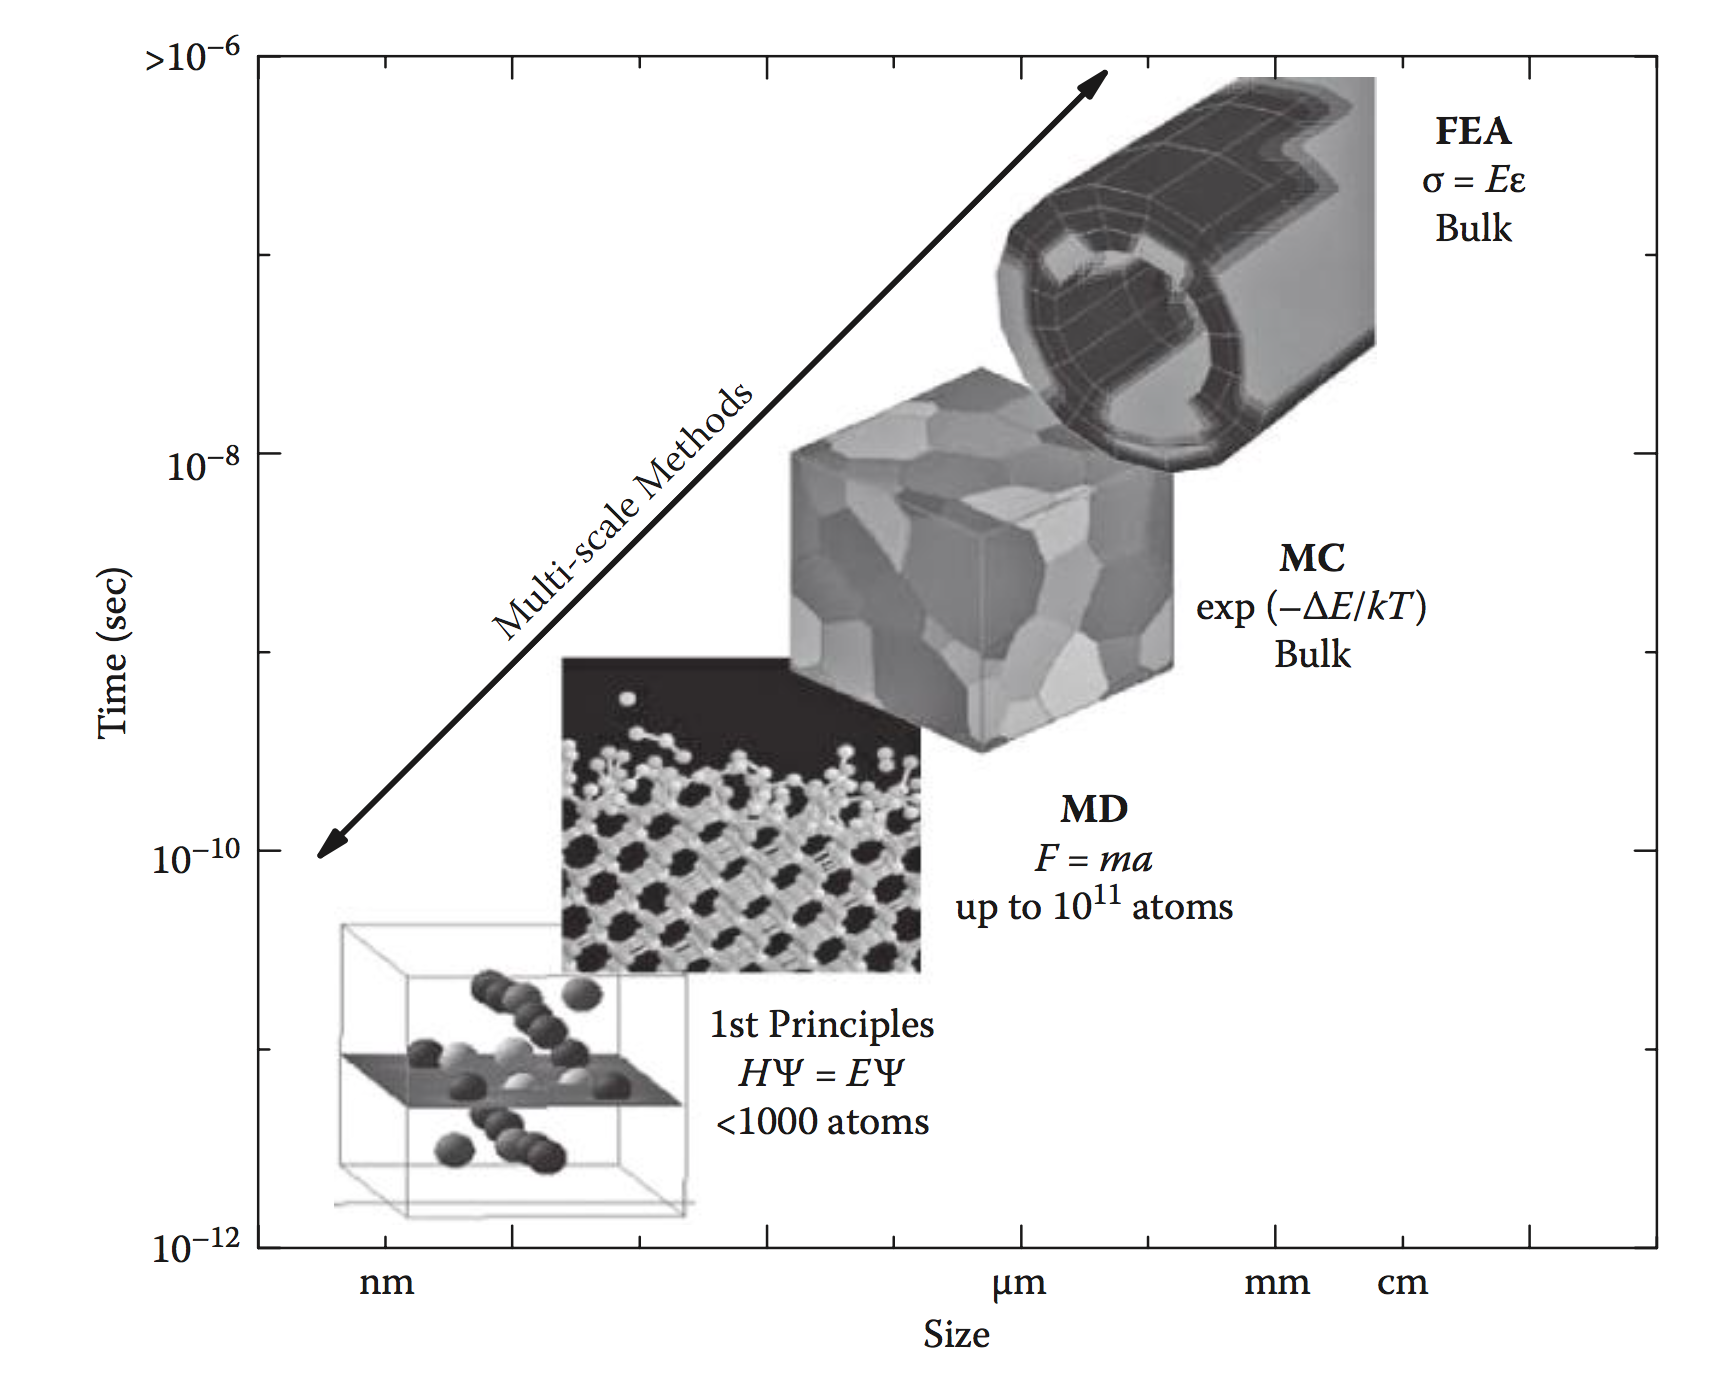
\includegraphics[width=0.5\textwidth]{overview}
	\centering
	\caption{Overview of computational methods with respect to time and size capabilities. \cite{Lee2012}}
\end{figure}





\section{Field Theory}

\section{Monte Carlo}

\section{Molecular Dynamics}

Molecular Dynamics (MD) is a classical method built off of

\begin{equation}
\vec{F}=m\vec{a} \qquad .
\end{equation}
Atoms are the smallest building block, represented as a sphere with a point mass \cite{Lee2012}. To calculate desired properties, atoms are allowed to ``relax" to their respective equilibrium distances, by moving down along the negative energy gradient:
\begin{equation}
\vec{F} = - \nabla U \qquad .
\end{equation}
A calculation begins with a set of starting atomic coordinates. The energy is calculated and the atoms are adjusted, following the gradient, to a more stable position. The energy is again calculated and compared to the previous step. This process continues until the differences between subsequent energy values reaches a predetermined stopping value, e.g. a difference of 1 $\times 10^-4$ eV or less.
\par
This method requires selection of so-called pair-potentials, which describe how atom $i$ interacts with atom $j$. The simplest potentail is the Lennard-Jones potential:

\begin{equation}
U_{ij}(r) = 4\epsilon \Bigg[\bigg(\frac{\sigma}{r}\bigg)^{12}-\bigg(\frac{\sigma}{r}\bigg)^{6}\Bigg] \qquad ,
\end{equation}
where $\epsilon$ is the depth of the energy well and $\sigma$ is the interatomic distance at which the potential is zero. However, this potential can only describe the interactions between atoms of the same element. In order to perform calculations on the majority of systems of interest, more complex pair-potentials are needed. Numerous potentials have been created, such as Embedded Atom Method (EAM) potentials which work for many metals and Tersoff potentials for covalent solids. 
\par 
An alternative method necessary for our discussion of AIMD in Section YYY is the Lagrangian:
\begin{equation}
L = K-U = \frac{1}{2}\sum_{i=1}^{3N}m_{i}v^{2}_{i}-U(r_{1}, \cdots, r_{3N})\qquad ,
\end{equation}
where $K$ is the kinetic energy, $U$ is the potential energy, and $N$ is the number of atoms.
\subsection{MD for the structure of alumina}
Guti\'errez et al. \cite{Gutierrez2002} used MD to investigate the structure of alumina. With the success of alloys and metals such as stainless steel, Ti, and Al largely attributed to their oxide layer, determining the structure of this oxide aids understanding of the passivation process. Guti\'errez used the pairwise potential
\begin{equation}
U(r_{ij})=\frac{q_{i}q_{j}}{r_{ij}}-\frac{C_{i}C_{j}}{r^{6}_{ij}}+D(B_{i}+B_{j})\exp\bigg(\frac{A_{i}+A_{j}-r_{ij}}{B_{i}+B){j}5}\bigg) \qquad ,
\end{equation}
where $r_{ij}$ is the interatomic distance between atoms $i$ and $j$, $D$ is the standard force constant 4.184 kJ/\AA$\cdot$mol., $q$ is the effective charge, $A$ is the repulsive radius, $B$ is the softness parameter, and $C$ is the van der Waals coefficient. This potential has been demonstrated to reproduce the structure, bulk modulus, thermal expansivities, melting temperatures, and liquid structure properties of Al$_{2}$O$_{3}$.
\begin{figure}[h]
	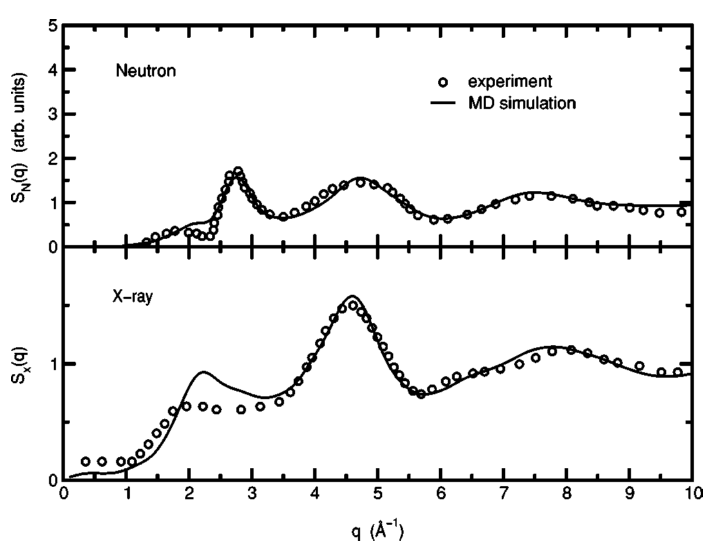
\includegraphics[width=0.6\textwidth]{gutierrez3}
	\centering
	\caption{MD results of Guti\'errez et al. \cite{Gutierrez2002} compared with experimental data for neutron and x-ray static structure function of Al$_{2}$O$_{3}.$} 
\end{figure}
\par
With a system of 1800 atoms, the researchers performed a melt-quench simulation by heating the system to 5000 K and evolving for 45 ps. Next the system was cooled to 3000 K at a rate of 1 K per 30 timesteps (1 fs). Finally, the system was allowed to equilibrate for 55 ps. Though these methods are known to be highly dependent on the melt-quench recipe, alternative initial configurations and quench rates were tested, but no discernible difference was found.
To perform statistical analysis of the structure, properties were averaged over 100 configurations: the last 100 structures, each 100 fs apart.

\begin{figure}[H]
	\centering
	\begin{minipage}[b]{0.45\textwidth}
		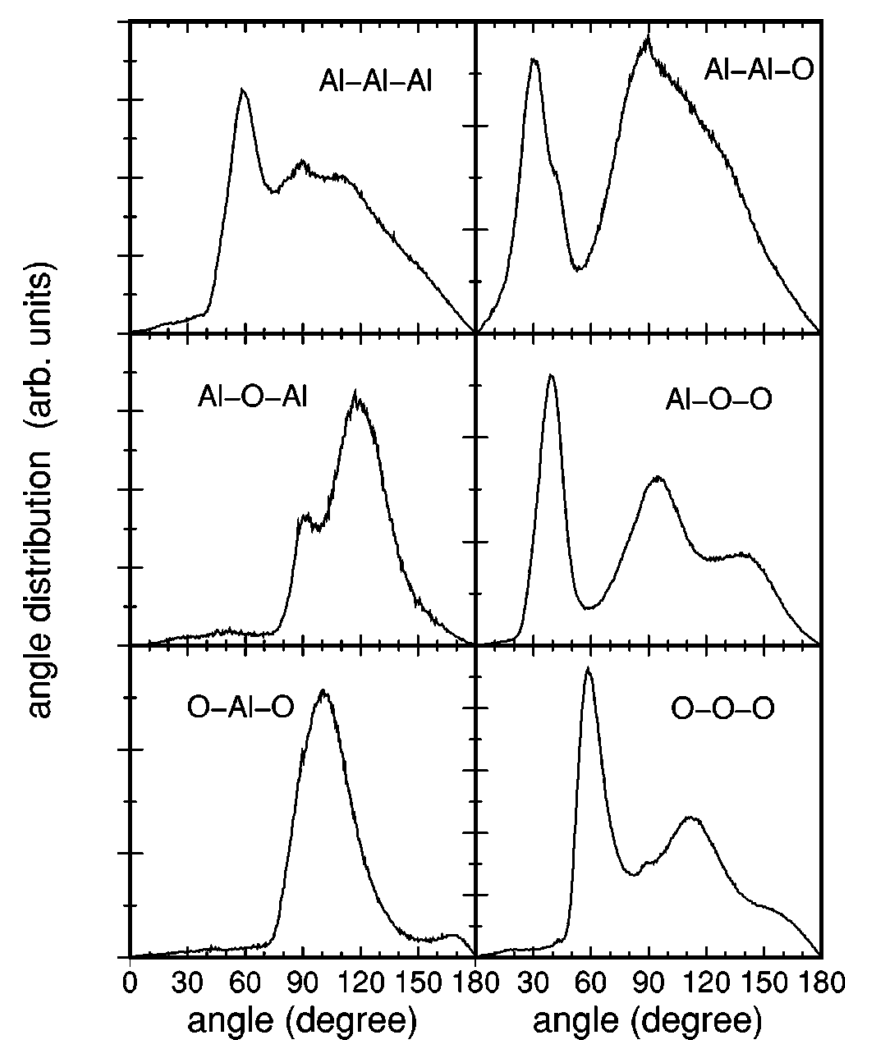
\includegraphics[width=0.94\textwidth]{gutierrez1}
		\caption{Results of Guti\'errez et al. \cite{Gutierrez2002} for bond angle distribution in amorphous Al$_{2}$O$_{3}$.}
	\end{minipage}
	\hfill
	\begin{minipage}[b]{0.45\textwidth}
		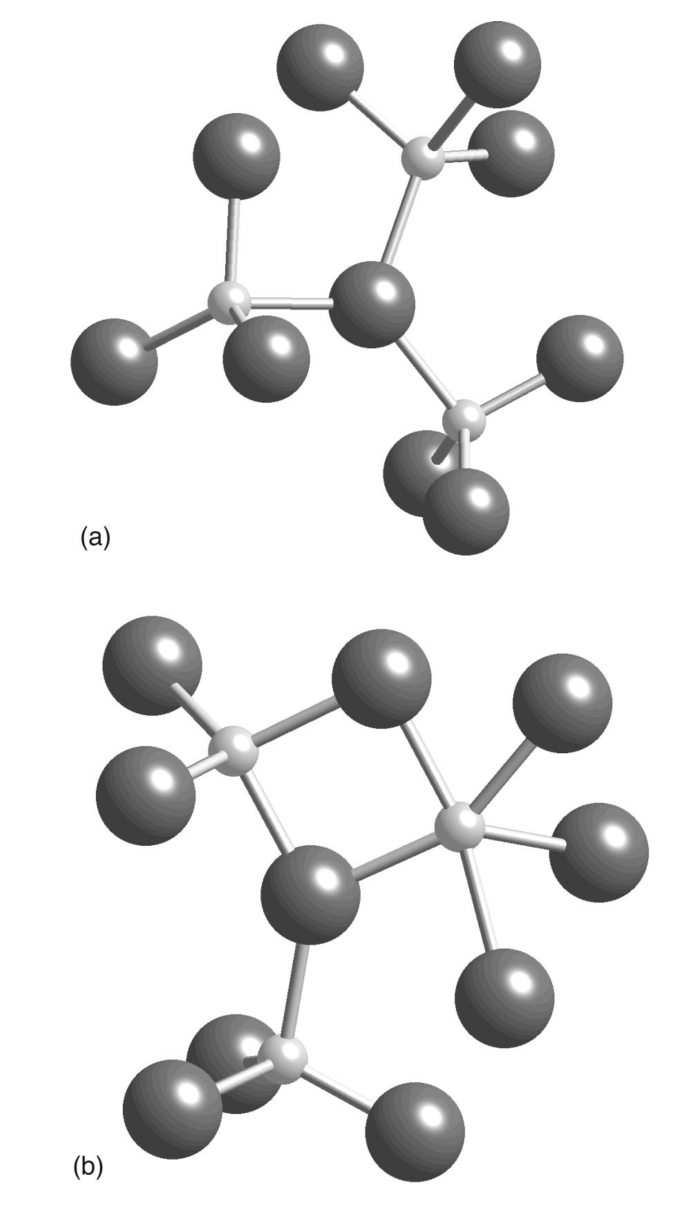
\includegraphics[width=0.55\textwidth]{gutierrez2}
		\centering
		\caption{Model suggested by Guti\'errez et al. \cite{Gutierrez2002} for basic Al$_{2}$O$_{3}$ units. (a) shows corner sharing tetrahedra while (b) shows edge-sharing polyhedra. Small and big spheres represent Al and O atoms, respectively. }
	\end{minipage}
\end{figure}
\par 
When compared with experimental structure factor, the results are in general agreement (Figure YYY). Though at low $q$ the results do not quite align, the simulation still shows a ``prepeak," consistent with experiment. From the bond-angle distribution shown in Figure YYY, the authors determined two structural motifs, as shown in Figure YYY.
%rings, gamma-alumina







\section{Density Functional Theory}
\begin{equation}
\hat{H}=-\frac{1}{2}\sum_{i}^{n}\nabla_{i}^{2}-\sum_{I}^{N}\sum_{i}^{n}\frac{Z_{I}}{|r_{Ii}|}+\sum_{i\neq j}^{n}\frac{1}{|r_{ij}|}
\end{equation}

\begin{equation}
\rho (r) = \sum_{i}|\phi _{i}(r)|^{2}
\end{equation}

\begin{figure}[H]
	\centering
	\begin{minipage}[b]{0.45\textwidth}
		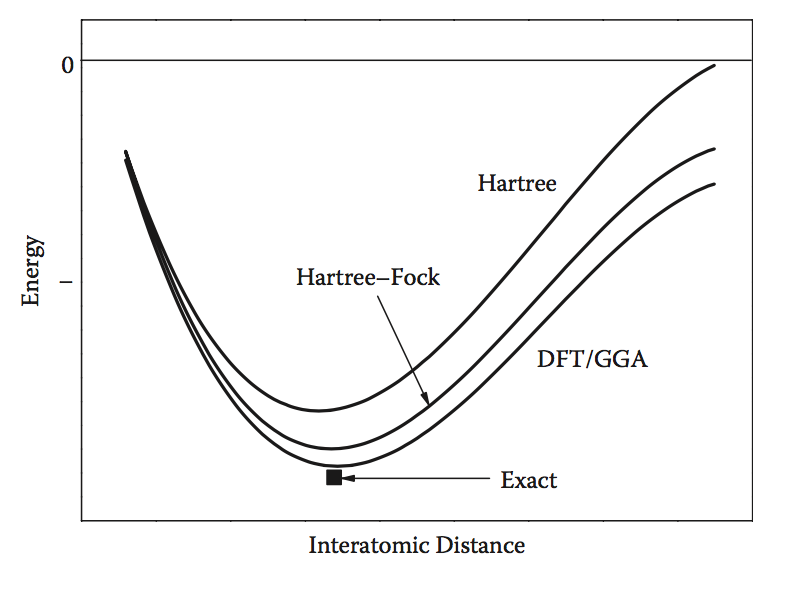
\includegraphics[width=\textwidth]{lee1}
	\end{minipage}
	\hfill
	\begin{minipage}[b]{0.45\textwidth}
		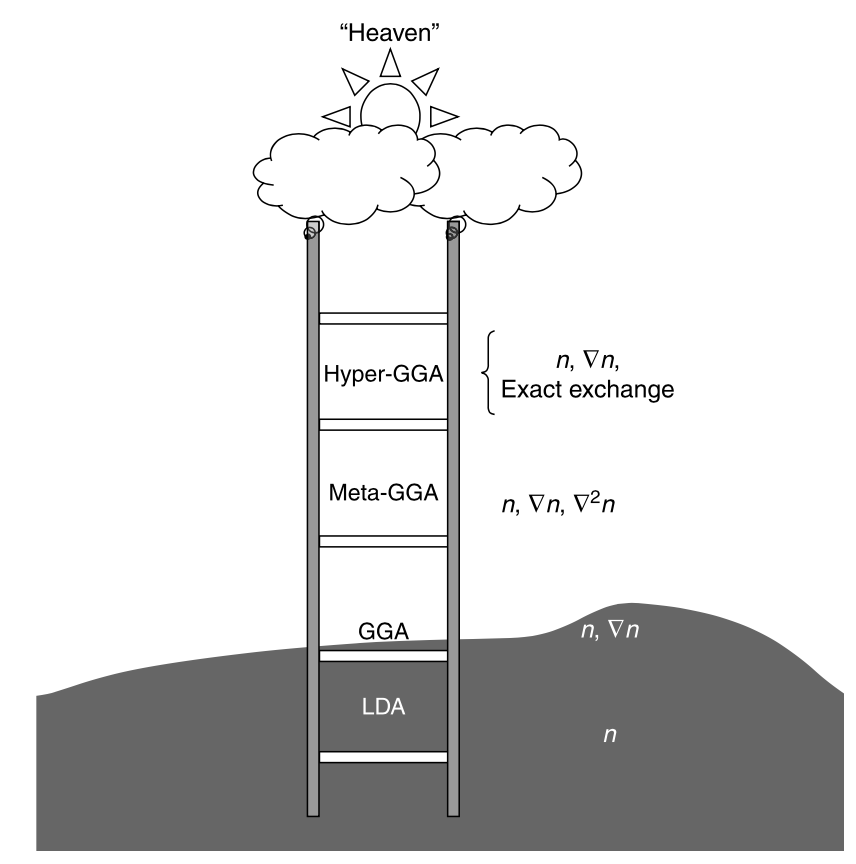
\includegraphics[width=\textwidth]{sholl1}
		\centering
	\end{minipage}
	\caption{Energy schematic \cite{Lee2012} (left) and Jacob's ladder depiction \cite{Sholl2009} of various functionals.}
\end{figure}
Meta-GGA, also referred to as hybrid functionals, combine Hartree Fock with DFT functionals. Going up the ladder represents increasing accuracy when compared with experiment, but it is done at computational cost. Any functional at the third rung or above is at least ten times as expensive as GGA \cite{Lee2012}. Though the Jacob's ladder is presented as a linear progression between functionals, this is a large simplification and the accuracy of a functional is often system-dependent. Another important consideration when selecting a functional is whether it is nonempirical - based on constraints of the Kohn-Sham functional - or empirical - parameterized by experiment \cite{Sholl2009}. The B3LYP functional, for example, is an empirical potential fitted to atomization energies, ionization potentials, and other experimental values \cite{Lee2012}. It excels in describing molecular systems, van der Waals interactions, and rapidly fluctuating electron densities. However, this method is not always well suited for metals and semiconductors \cite{Paier2007}.

\subsection{Photoluminescence in amorphous perovskites}
\begin{figure}[h]
	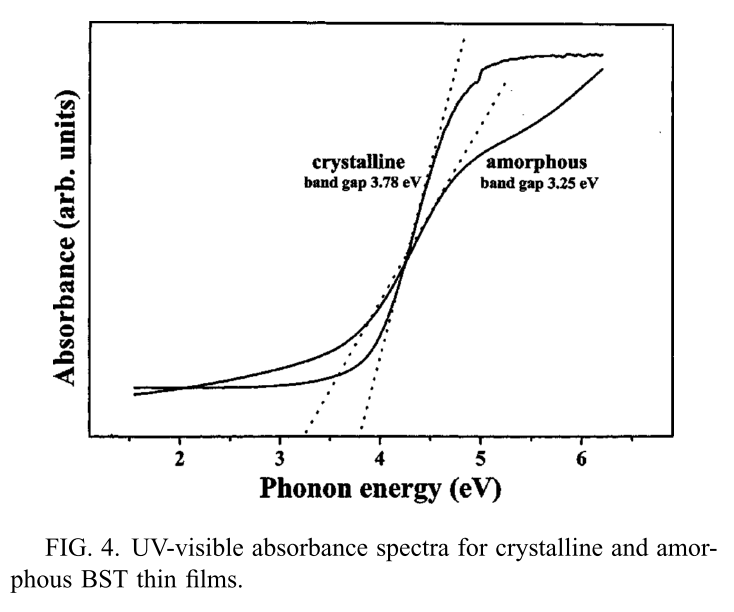
\includegraphics[width=0.6\textwidth]{longo3}
	\centering
	\caption{UV-visible absorbance spectra for crystalline and amorphous Ba$_{0.5}$Sr$_{0.5}$TiO$_{3}$ films from Longo et al. \cite{Longo2004}} 
\end{figure}
Longo et al. \cite{Longo2004} used DFT to determine the origin of photoluminescence in their amorphous titanates. They chose  crystalline and amorphous Ba$_{0.5}$Sr$_{0.5}$TiO$_{3}$ (BST) for computational analysis using the B3LYP functional. From x-ray absorption near edge spectra (XANES), they determined the amorphous titanates contained both fivefold and sixfold oxygen-titanium coordination. In order to create this coordination, they shifted the Ti atom by 0.5 $\AA$, as shown in Fig. YYY. From the band gap in Fig. YYY, the indirect bandgap in crystalline BST is equal to 3.78 eV, in agreement with the optical bandgap found in experiment (Figure. YYY). For amorphous BST, this indirect bandgap decreases to 3.06 eV. The LDOS in Fig. YYY show the valence band is made up of O states while the conduction band is made of Ti states. The authors note covalent bonding occurs between Ti and O, through the overlap of Ti 3d states and O 2p states. The nature of the bonding is further realized in Fig. YYY(a). A  valley exists in the surface plot between Ba and Sr, indicating ionic bonding. Conversely, the charge density between Ti and O is higher and can additionall by seen in the contour map as exhibiting regions of the same charge. These characteristics point to covalent bonding. Fig. YYY(b) emphasizes the distinction between the Ti-O bonds in crystalline an amorphous BST: the covalent bonds are weaker in amorphous BST as the contour map shows reduced regions of the same charge density. These results suggest that the change in the Urbach tail of the absorption spectra is due to the disorder in the amorphous structure which leads to localized states in the O 2p orbitals.
\begin{figure}[H]
	\centering
	\begin{minipage}[b]{0.45\textwidth}
		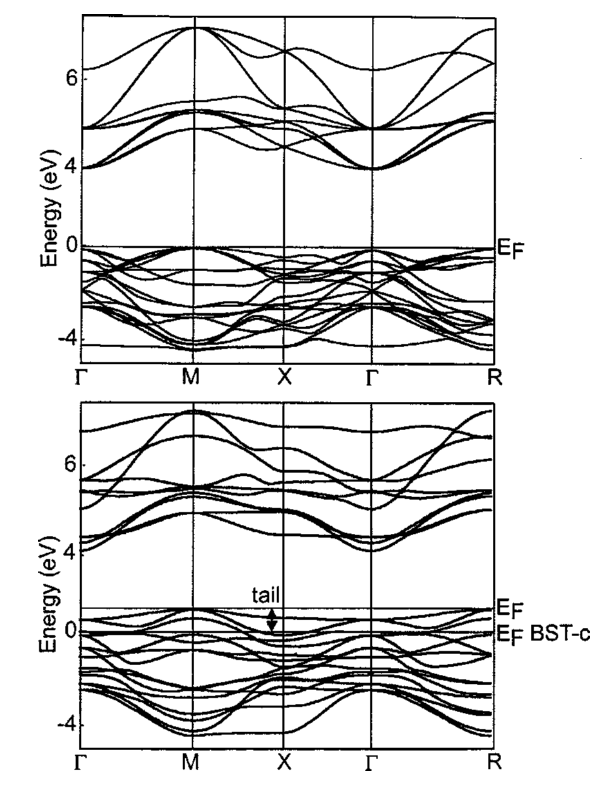
\includegraphics[width=\textwidth]{longo1}
	\end{minipage}
	\hfill
	\begin{minipage}[b]{0.45\textwidth}
		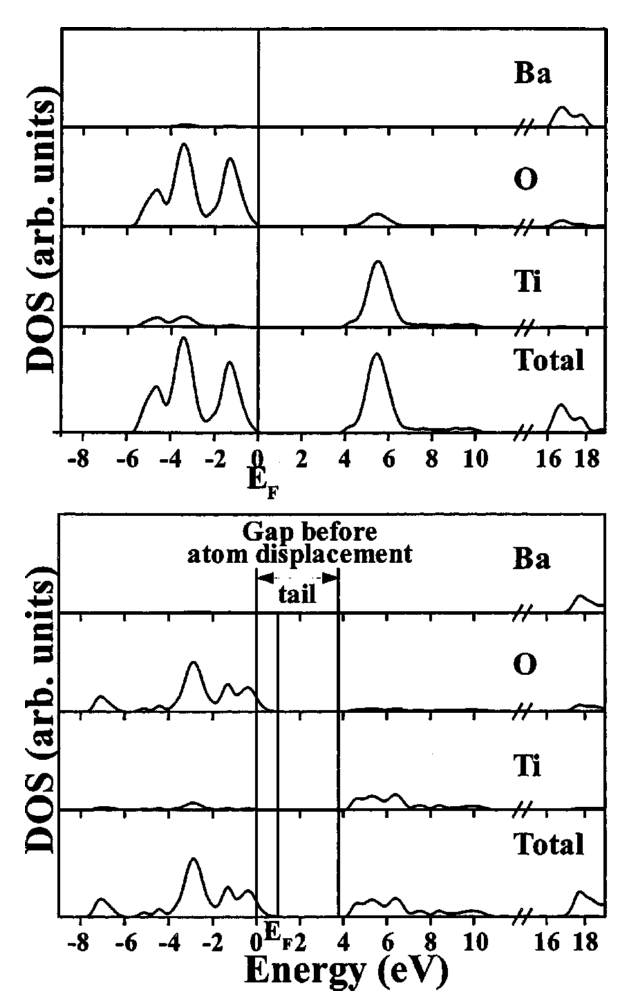
\includegraphics[width=0.82\textwidth]{longo2}
		\centering
	\end{minipage}
	\caption{Calculated band structure (left) and density of states (right) from Longo et al. \cite{Longo2004} for crystalline (top) and amorphous (bottom) Ba$_{0.5}$Sr$_{0.5}$TiO$_{3}$.}
\end{figure}



\begin{figure}[H]
	\centering
	\begin{minipage}[b]{0.45\textwidth}
		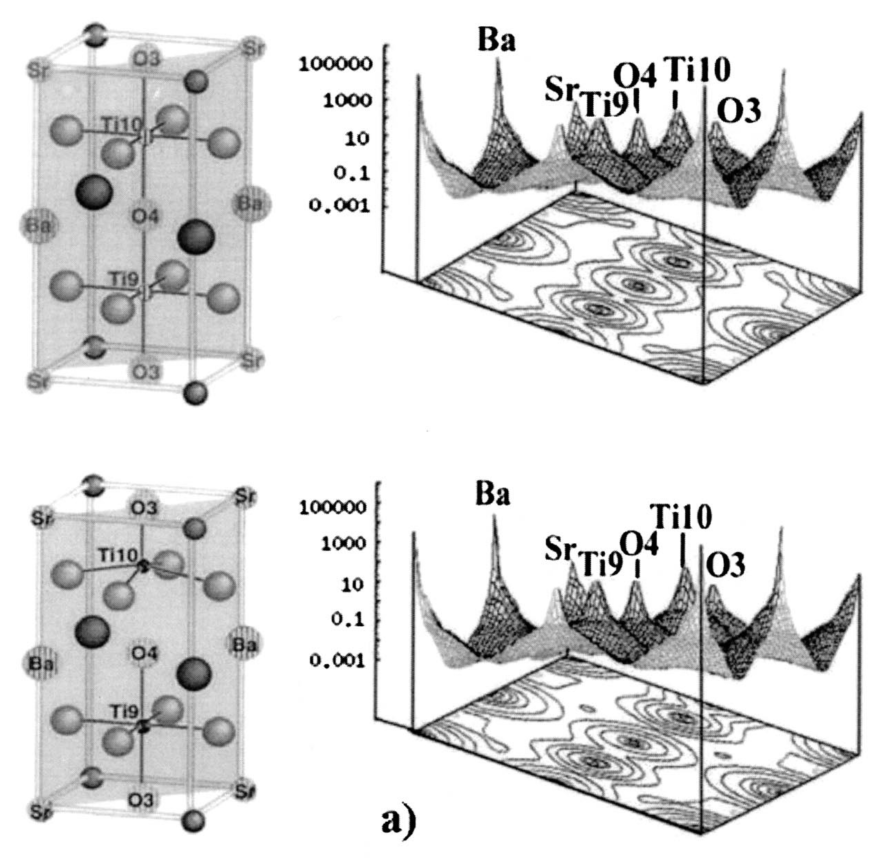
\includegraphics[width=\textwidth]{longoA}
	\end{minipage}
	\hfill
	\begin{minipage}[b]{0.45\textwidth}
		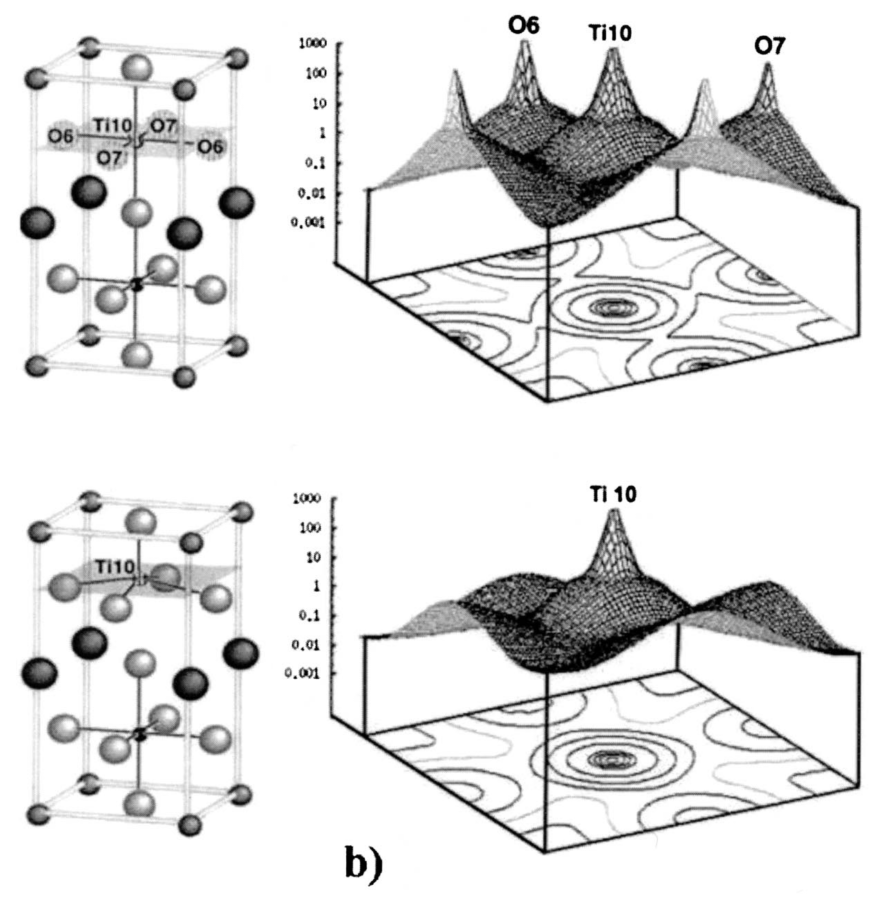
\includegraphics[width=0.95\textwidth]{longoB}
		\centering
	\end{minipage}
	\caption{Charge density from surface and contour plots from Longo et al. \cite{Longo2004} for crystalline and amorphous  Ba$_{0.5}$Sr$_{0.5}$TiO$_{3}$. (a) shows the vertical diagonal plane and (b) shows a horizontal plane.}
\end{figure}

\par

Though the band gap results of Longo et al. agree well with their experimental data, the structure they modeled is not entirely amorphous. Due to their small unit cell of 1 $\times$ 1 $\times$ 2, this creates a periodic structure in which half of the Ti have distorted local bonding. If there were greater distribution of bond lengths and types, it is likely further details in the photoluminescence mechanism could be unearthed.
\par

Additionally, the B3LYP is a partially empirical functional \cite{Paier2007}. Due to the fixed nature of empirical potentials, this method may struggle in accurately representing the system if the system exhibits any anisotropy \cite{Hohl1991}. Paier et al. \cite{Paier2007} have shown that B3LYP performs poorly for metals and small gap semiconductors, which would be better described with nonempirical hybrid functionals such as PBE0 and HSE03. At the high computational cost of a hybrid functional, a nonempirical functioanl may be better suited for this study.














\section{\emph{Ab intio} Molecular Dynamics}
\emph{Ab initio} Molecular Dynamics (AIMD) refers to any calculation that advances atoms along classical trajectories based on forces calculated from DFT\cite{Sholl2009}.
\par 
AIMD is an incredibly powerful method capable of adding time to a DFT simulation while still allowing for \emph{ab initio} calculation of electronic properties. Furthermore, AIMD can circumvent the problem of metastable states, as shown for DFT+U \cite{Zhang2015}. This can be better conceptualized with the schematic of Car-Parrinello MD in Figure YYY. Instead of performing AIMD as a stepwise process in which calculating the atomic trajectories and the electronic ground state are separate, Car and Parinello formulated the two to run simultaneously. Their extended Lagrangian introduces the electronic degrees of freedom as fictitious dynamical variables:
\begin{equation}
L =\frac{1}{2}\sum_{i=1}^{3N}m_{i}v^{2}_{i}-U(r_{1}, \cdots, r_{3N})+\frac{1}{2}\sum_{j}2\mu \int d\vec{r}|\dot{\psi}(\vec{r})|^{2}+L_{ortho}
\end{equation}
The third term introduces fictitious mass, $\mu$, and the final term restrains the one-electron wave functions to be orthogonal. Since the total energy calculation occurs simultaneously with the atomic trajectory calculation, the energy is not quite the same as the energy calculated with pure DFT, as shown in Figure YYY. This phenemona circumvents the structure getting trapped in a metastable state, as DFT methods are known to do \cite{Dorado2013}.
\begin{figure}[h]
	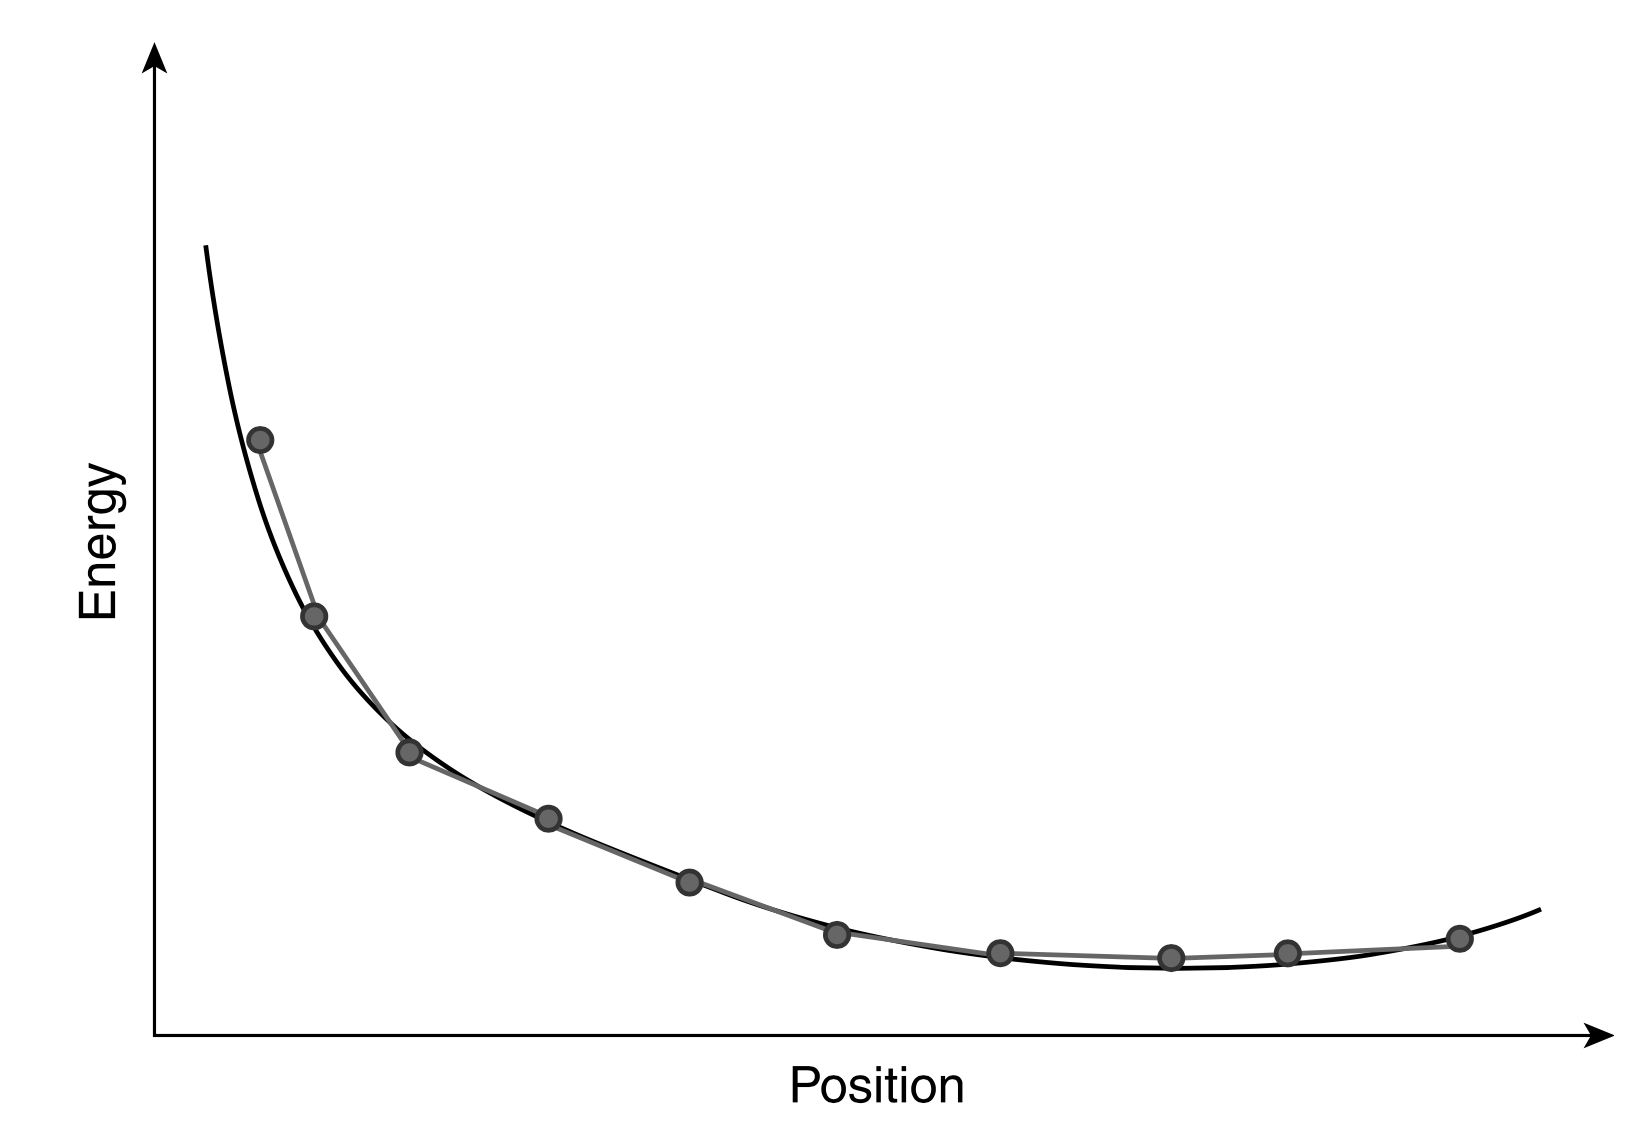
\includegraphics[width=0.5\textwidth]{practical1}
	\centering
	\caption{} 
\end{figure}

\par
Shortly after the formulation of Car-Parrinello MD, Car and Parrinello realized the utility of the method for 

\subsection{AIMD for Phase Change Memory}
Raty et al. \cite{Raty2015} used Ab Initio Molecular Dynamics to understand the structural changes associated with aging in GeTe, and the effects those changes have on performance. Inherently out of equilibrium, amorphous materials evolve with time to a lower energetic state. In the case of phase change materials, this evolution leads to higher electrical resistivity that undermines its usability in multilevel memory devices. Using AIMD, we can watch the structure evolve, but though we discussed the addition of time to DFT above, this time is still on the order of picoseconds, leaving real-time aging out of the quesion. Raty et al. have sidestepped this problem by creating an arrangement of structures with varying local motifs. 
\par
Their study begins with the observation that AIMD simulations of Ge$_{x}$Sb$_{y}$Te$_{1+x+y}$ alloys show tetrahedrally bonded Ge (Ge$^{T}$) atoms in the amorphous phase, though these are absent in crystalline Ge. To investigate the effect of such homopolar bonds on GeTe properties, the authors melt-quenched GeTe along with a combination of other binary chalcogenides for use as``templates." SiTe forms numerous Si$^{T}$, GeSe contains some Ge$^{T}$, and SnTe contains almost no tetrahedral motifs.  The authors then substituted one species in each of the template compounds to form GeTe, i.e. substituting Si in SiTe with Ge, Se in GeSe with Te, and Sn in SnTe with Ge. After substitution, the systems were subjected to a shorter additional melt-quench procedure.
\begin{figure}[h]
	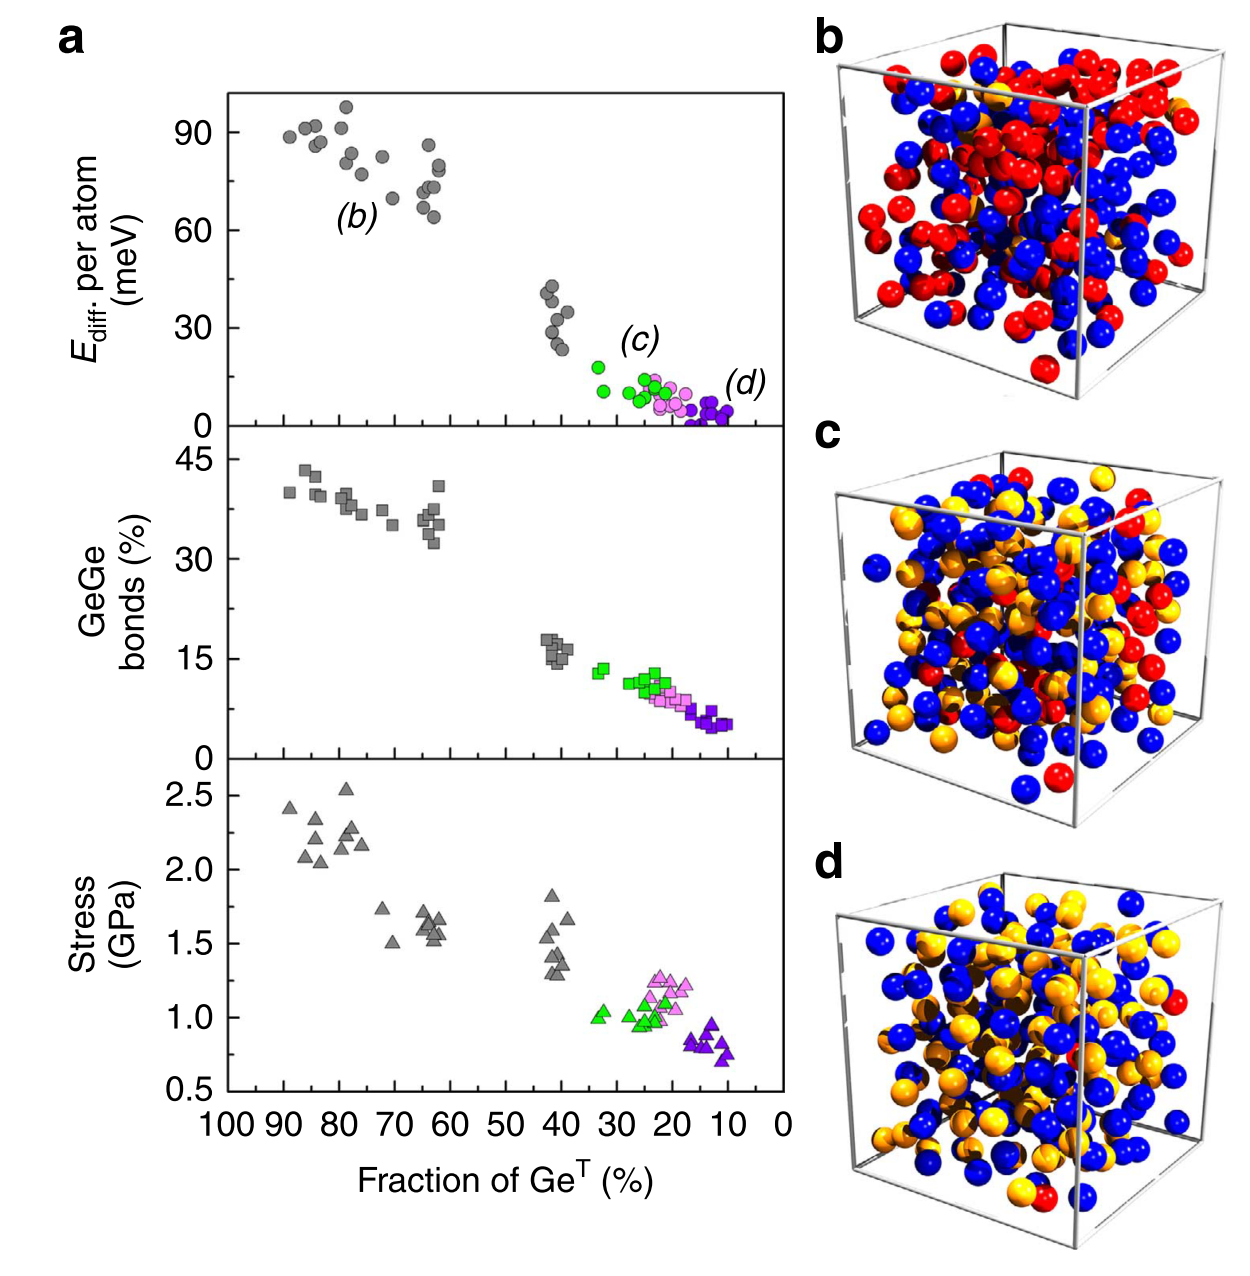
\includegraphics[width=0.5\textwidth]{raty1}
	\centering
	\caption{Results from Raty et al. \cite{Raty2015} for (a) the energy difference per atom, fraction of homopolar GeGe bonds, and stress of the melt-quenching of GeTe (green) and chemical replacement systems SnTe (violet), GeSe (pink), and SiTe (grey). (b-d) show the atomic configurations of GeTe as labeled in the energy difference plot. Te, tetrahedral Ge, and octahedral Ge are rendered in blue, red, and orange, respectively.} 
\end{figure}
\par 
The results shown in Figure. YYY indicate that the homopolar bonds reduce the stability of the system. However, homopolar bonds have a lower heat of formation in GeTe than in both GeSe and SnTe, and the melt-quench process is able to stabilize these tetrahedral motifs. In comparison to experiment, aging of phase change materials has been linked with stress relief. These results suggest that the removal of homopolar bonds contributes to this stress relief.
\par 
Raty et al. additionally calculated the changes in the electronic and optical bandgaps due to the changes in percent Ge$^{T}$. Though methods of calculating optical properties are beyond the scope of this review, the results of Raty et al. for the optical bandgap in Figures. YYY(a) and YYY show increasing band gap correlated with decreasing homopolar bonds, in agreement with experiment showing band gap widening with aging. Similarly, the DOS shows an increase in electronic band gap with aging, and the disappearance of the midgap states are directly linked to the removal of homopolar bonds. The authors note that while a variety of Ge$^T$ concentrations have been modeled, this method does not yield access to the time scale of the relaxation process. 
\begin{figure}[h]
	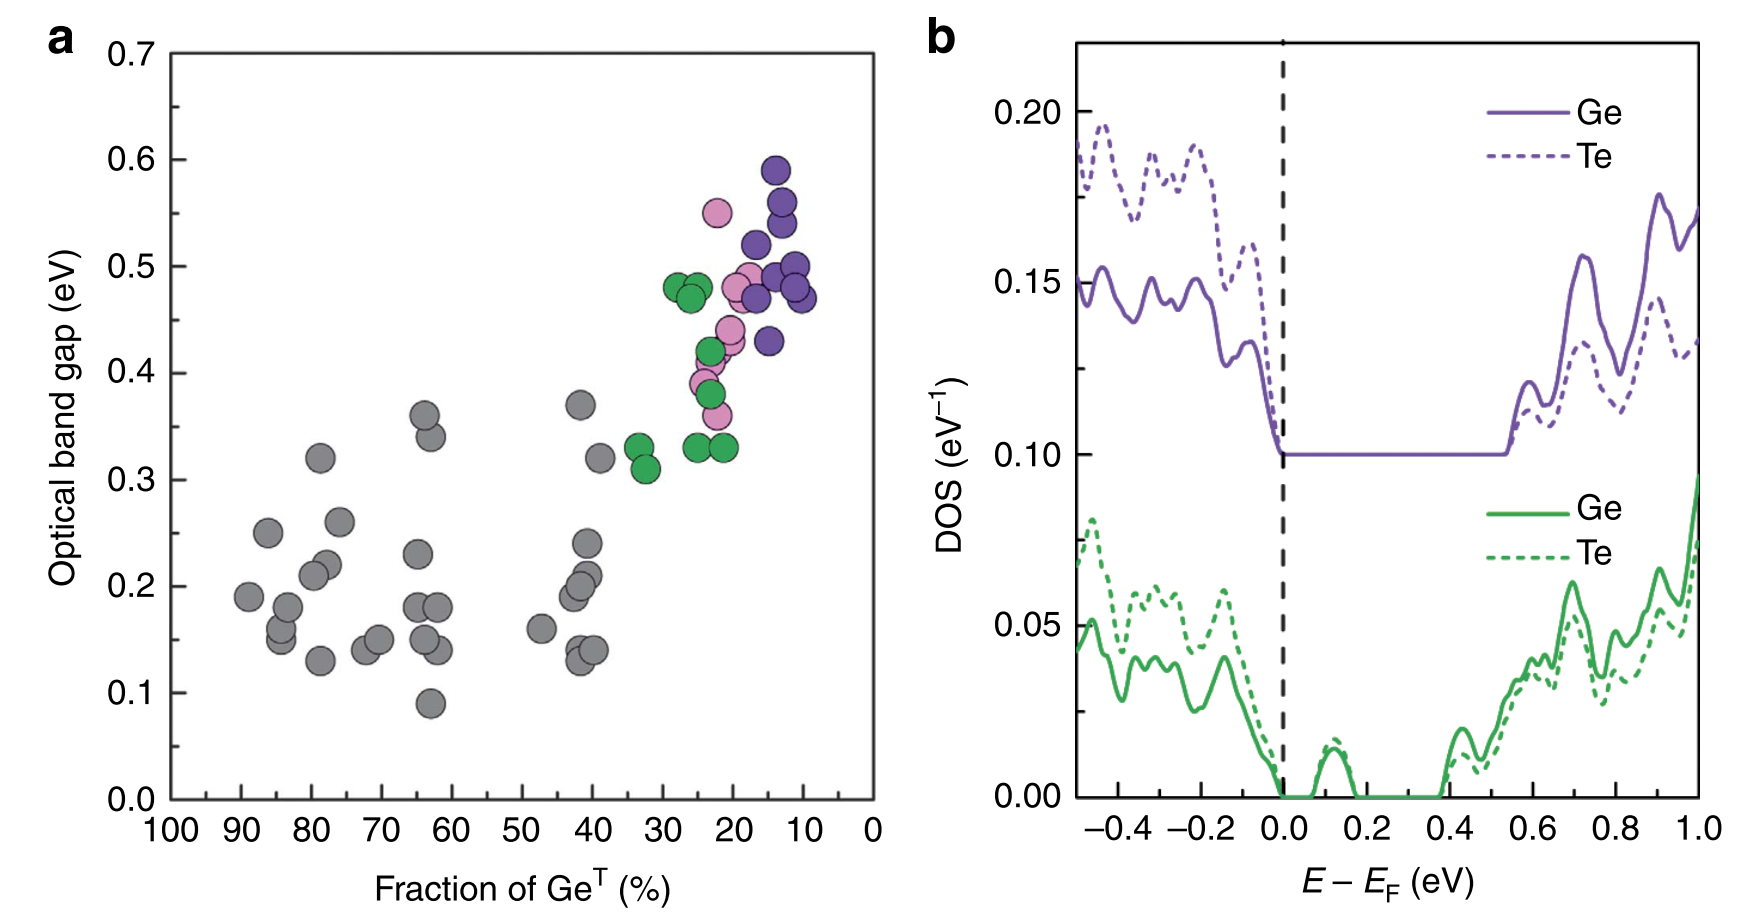
\includegraphics[width=0.5\textwidth]{raty2}
	\centering
	\caption{Results from Raty et al. \cite{Raty2015} for (a) the relaxed amorphous GeTe structures as a function of percent Ge$^{T}$} and (b) the local density of states for melt-quenched GeTe (green) and substituted a-SnTe (violet).
\end{figure}
\begin{figure}[h]
	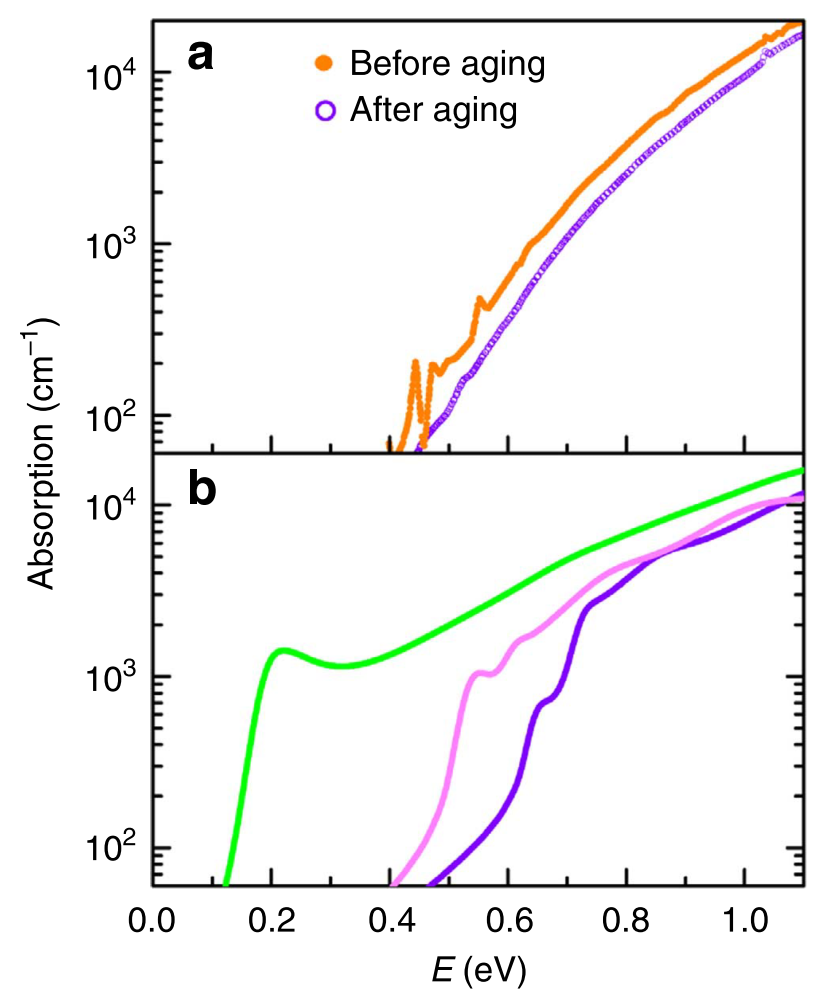
\includegraphics[width=0.3\textwidth]{raty3}
	\centering
	\caption{Results from Raty et al. \cite{Raty2015} for (a) experimental absorption from photothermal deflection spectroscopy (PDS) and (b) calculated absorption oscillator strength for melt-quenched GeTe (green), substituted a-GeSe (pink), and substituted a-Sn-Te (violet). } 
\end{figure}

\subsection{Example AIMD melt-quench run}

\section{Conclusion}
know when your methods fail
\begin{itemize}
	\item MD iff
	\begin{itemize}
		\item isotropic
		\item potential reproduces desired properties
	\end{itemize}
\end{itemize}




\pagebreak

\section*{Notes}

\begin{itemize}
	\item Kohn Sham: A \emph{system} of one-electrons
	\item Hartree: a \emph{potential} of how each electrons feels the electron gas
	\item Hartree Fock: how we describe the wave functions
\end{itemize}
\subsection{AIMD}
\underline{Hohl 1991}\cite{Hohl1991} - Liquid and amorphous Se \par \vs
\textbf{Computational comments}
\begin{itemize}
	\item many structural models have been proposed and often conflict
	\item models based solely on small differences are insufficient to explain all measured features
	\item even carefully constructed empirical potentials have difficulty in highly anisotropic covalent systems such as group-IVA elements.
	\item AIMD avoids parameterization of interatomic forces common in MD
\end{itemize}

\underline{Raty 2015 \cite{Raty2015}} - Aging in Phase Change Materials (dots figure)
\par
\begin{itemize}
	\item Motivation
	\begin{itemize}
		\item "Amorphous materials are out of thermodynamic equilibrium"
		\item subject to physical aging
		\item phase-change materials (PCMs) have a fast, reversible switch between a conductive crystalline and more resistive amorphous phase
		\item aging increases the resistivity - `resistance drift'
		\item computer simulation to investigate relaxation processes
		\item \textbf{Modeling comment:} complexity of the chemistry requires DFT to describe and understand bonding and the amorphous phase
	\end{itemize}
	\item Literature
	\begin{itemize}
		\item DFT simulations of GeSbTe alloys report many tetrahedrally bonded Ge, which does not exist in crystal. These are obtained from MQ calcs
	\end{itemize}
	\item Methods
	\begin{itemize}
		\item Car-Parrinello
		\item \textbf{To circumvent time scale problem, generated collection of a-structures}
		\item mixed Gaussian/plane wave code in CP2K
		\item cutoff 300 Ry
		\item sampled at gamma only
		\item annealed using plane-wave code in Quantum Espresso
		\item 34 Ry
		\item 3.84 fs
		\item Berendsen thermostat
		\item 10 models produced starting from liquid
	\end{itemize}	
	\item Results
	\begin{itemize}
		\item Ge$^{T}$ is associated with homopolar Ge-Ge bonds
		\item heat of formaion shows homopolar bonds more favorable in GeTe than GeSe and SnTe
		\item wanted to investigate effects of varying amounts Ge-Ge bonds
		\item used different alloys along the phase diagram and substituted with Ge or Te to form different GeTe structures "mimicking aging"
		\item homopolar bonds correlated with tetrahedral Ge
		\item freezing at density of amorphous GeTe, tetrahedral rich models had the largest values of stress
		\item this agrees with experiments showing the drift of PCMS is accompanied by stress relief
		\item order parameter $d_{4}/d_{0}$ goes from tetrahedrally bonded Ge, $Ge^{T}$, to $Ge^{III}$ and $d_{3}/d_{0}$ goes from $Te^{II}$ to $Te^{III}$
		\item increase in band gap directly linked to decrease in homopolar bonds
		\item "melt-quenched model has a smaller band gap and possesses a (localized) mid-gap state"
	\end{itemize}	
\end{itemize}



\section*{References}

\bibliography{amorph}
\bibliographystyle{elsarticle-num}

\end{document}  